\chapter{Обзор литературы}



\section{Вариабельность сердечного ритма }

Вариабельность сердечного ритма (Heart rate variability) это явление изменения частоты сердечного ритма.

Вариабельность сердечного ритма очень сильно зависит от эмоционального \cite{hrv_and_sensitivity, hrv_and_respiratory} и физического \cite{hrv_and_phisical_health} здоровья человека и может использоваться как его показатель.

Существуют два основных частоты колебания сердечного ритма \cite{two_rates_hrv}.

\begin{itemize}
	\item Колебания, вызванные дыхательной аритмией. При этом частота сердечных сокращений изменяется в связи с дыханием и можно отследить частоту дыхания.
	\item Низкочастотные колебания артериального давления. Это явление называется волнами Майера \cite{mayer_wave} артериального давления и, как правило, имеют частоты порядка 0,1 Гц.
\end{itemize}

Для наблюдения за сердечным ритмом применяются следующие методы:

\begin{itemize}
	\item ЭКГ (электрокардиография) \cite{EKG};
	\item баллистокардиография  \cite{Ballistocardiograms};
	\item фотоплетизмография \cite{Photoplethysmography}.
\end{itemize}

ЭКГ считается методом, дающим наиболее четкий сигнал.

\subsection{ЭКГ}

Электрокардиография измеряет электрическую актовность сердца за некоторый период времени с помощью электродов, наложенных на различные участки сердца. Электроды сквозь кожу регистрирую слабый электрический сигнал, вызываемый серцебиением. Обычно 10 электродов располагаются на груди и конечностях пациента. С их помощью измеряются общая величина электрического потенциала и его направление. График зависимости потенциала от времени называется электрокардиограммой. Ее пример можнео увидеть на рис. \ref{ris:RR}.

\begin{figure}[h]
\begin{center}
	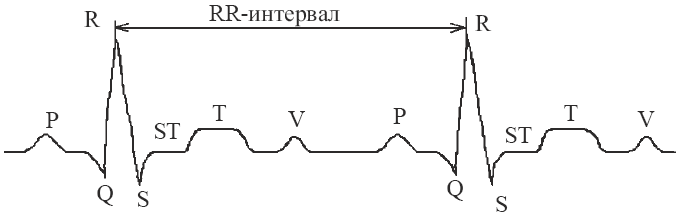
\includegraphics[scale=0.36]{RR.png}
	\caption{ЭКГ}
	\label{ris:RR}
\end{center}
\end{figure}

RR-интервалом называется промежуток времени между последовательными ударами сердца. Нормально частотой серцебиения считается 60-100 ударов в минуту в состоянии покоя. Если рассматривать момент сокращения сердца более подробно \cite{polarization_heart} виден QRS-комплекс - изменения электрического потенциала, предшествующее сокращению сердца.а электрической активацией клеток (деполяризацией) следует механическое сокращение, создаваемое следующим образом. Процесс сокращения сердечных мыщц состоит из следующих стадий.

\begin{itemize}
	\item деполяризация предсердий; зубец P
	\item передача импульса желудочкам; интервал PR
	\item деполяризация желудочков; зубец R
	\item реполярицазия желудочков; зубец T
	\item мнения исследователей относительно причин происхождения зубца V различны
\end{itemize}

\subsection{Обработка ЭКГ}

\subsection{анализ HRV}

Основные методы исследования HRV.

\begin{enumerate}
	\item Методы основанные на анализе интервалов между сердечными ударами NN типа. При данном анализе часто подсчитываются следующие характеристики \cite{pNN, metric_of_hrv}.
	\begin{enumerate}
		\item SDNN, стандартное отклонение интервалов NN от среднего, вычесленого почти всегда в течение 24 часов. SDNN обычно вычисляется для коротких интервалов, порядка 5 минут. SDNN отражает все циклические компоненты, ответственные за изменчивость в период записи, поэтому она представляет собой общую вариабельность.
		\item 	RMSSD ("среднеквадратичное последовательных различий»), квадратный корень из среднего значения квадратов последовательных разностей между соседними NN ударами.
		\item SDSD ("стандартное отклонение последовательных разностей"), стандартное отклонение последовательных разностей между соседними NNS.
		\item NN50, количество пар последовательных NN ударов, которые отличаются более чем 50 мс.
		\item pNN50, доля NN50 делится на общее количество NN ударов.
		\item 	NN20, количество пар последовательных NN ударов, которые отличаются более чем 20 мс.
		\item pNN20, доля NN20.
		\item EBS ("оценивается цикл дыхания"), диапазон (макс-мин) в скользящем окне заданной длительности. Окна можно перемещать без перекрытия или с перекрытием. ЕВС часто используют при сборе данных, где обратная связь ВСР в режиме реального времени является главной целью.
	\end{enumerate}
	\item Геометрические методы \cite{geometric_metric}
	\item Частотный анализ
	
	Строятся гистограммы частотных характеристик NN ударов
	
	\item Подсчет кореляций следующих NN ударов от предидущих \cite{autocorr_metric}
	\item Нелинейные методы \cite{non_linear_metric}
	
	\begin{enumerate}
		\item график Пуанкаре \cite{poinkare_plot}.
		\item фрактальные размерности \cite{fractal_dim}.
		\item флуктуационный анализ \cite{fluct_analis}
		\item энтропия \cite{entropy1, entropy2, entropy3}
		\item и др. \cite{other_analis1, other_analis2, other_analis3}
	\end{enumerate}	
\end{enumerate}

\section{Рекуррентные нейронные сети}
Рекуррентная нейронная сеть – один из типов нейронных сетей \cite{neural_network}, в котором присутствует обратная связь. Другими словами в выход более позднего слоя сети поступает на вход более слоя, считающегося ранее.

Рекуррентные нейронные сети имеют ряд преимуществ перед обычными.
\begin{itemize}
	\item Разнообразные виды входных данных
	\item Способность строить неявные модели данных
	\item Устойчивость к выбросам
	\item 
\end{itemize}

Рекуррентные сети применяются в таких задачах как:
\begin{itemize}
	\item распознавание устной и письменной речи \cite{rnn_for_speech_recognition, rnn_for_text_recognition};
	\item машинный перевод \cite{rnn_for_translation};
	\item предсказания временных рядов \cite{rnn_for_prediction};
	\item И т.п.
\end{itemize}



Основной проблемой при использовании рекуррентных нейронных сетей является проблема исчезающего градиента (vanishing gradient problem \cite{vanishing_gradient_problem}). Если честно подсчитывать градиент на каждой итерации обучения он будет выражаться через произведение градиентов, подсчитанных на всех предыдущих итерация. Если градиенты были малы – наш градиент будет просто не заметен и обучение встанет надолго. 

Проблема исчезающего градиента была подробно рассмотрена Хочрайтером???(произношение) and Шмидхубера, которые разработали LTSM архитектуру \cite{create_lstm}, которая устойчива к данной проблеме. Данная архитектура оказалась проста в использовании и стала стандартным средством борьбы с исчезающим градиентом. Также были осуществлены попытки других способов решения данной проблемы:
\begin{itemize}
	\item обратное распостранение во времени (Backpropagation through time) \cite{Backpropagation}. Используется для обучения сетей Элмана.
	\item использование мощного secondorder алгоритмы оптимизации (Martens, 2010; Мартенс Sutskever, 2011)
	\item регуляризация весов в RNN, что гарантирует, что градиент не обращается в нуль (Pascanu др.,2012)
	\item отказ от всего обучения текущие веса (Jaeger, Haas, 2004; Jaeger, 2001), и очень
	осторожны инициализации параметров РНН (в Sutskever др.,2013).
\end{itemize}
	
Также была обнаружена проблема сильного возрастание градиента, но она легко решилась ограничение на модуль градиента.

\subsection{LSTM}

Данный слой успешно борется с проблеммай исчезающего градиента. Каждый нейрон в данном слое представняет собой "ячейку памяти" (рис. \ref{ris:ltsm}). Данные ячейки организованны для хранения информации и позволяют более качествеено обрабатывать длинные входные последовательности.

\begin{figure}[h]
\begin{center}
	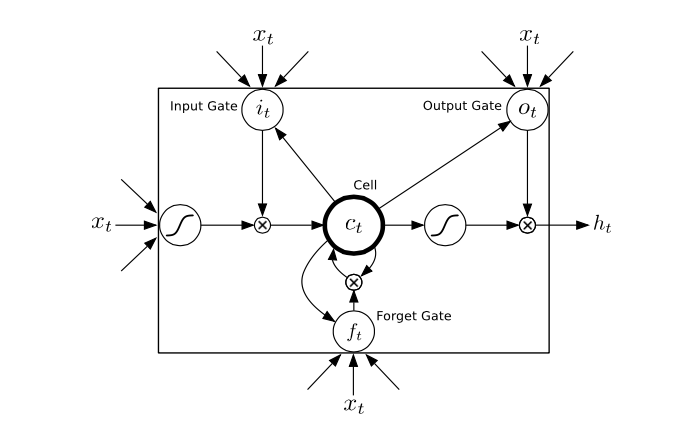
\includegraphics[scale=0.36]{ltsm.png}
	\caption{LSTM ячейка}
	\label{ris:ltsm}
\end{center}
\end{figure}


Пускай на вход LSTM ячейке памяти подается часть входной последовательности $x_t = (x_1, ..., x_N)$ и предыдущие выходной вектор признаков $h_{t-1} = (h_1, ..., h_M)$. Ячейка должна подсчитать вектор признаков $h_t$. Ячейка организованны следующим обрахом:


\begin{equation}
	i_i = \sigma(W_{xi}*x_t+W_{hi}*h_{t-1}+W_{ci}*c_{t-1}+b_i)
\end{equation}
\begin{equation}
	f_t = \sigma(W_{xf}*x_t+W_{hf}*h_{t-1}+W_{cf}*c_{t-1}+b_f)
\end{equation}
\begin{equation}
	c_t = f_t*c_{t-1}+i_t*\tanh(W_{xc}*x_{t-1}+W_{hc}*h_{t-1}+b_c)
\end{equation}
\begin{equation}
	o_t = \sigma(W_{xo}*x_t+W_{ho}*h_{t-1}+W_{co}*c_t+b_o)
\end{equation}
\begin{equation}
	h_t = o_t*\tanh(c_t)
\end{equation}

Здесь $\sigma = \frac{1}{1+e^{-x}} $ - сигмоида, логистическая функция, принимающая значения от 0 до 1. А i, f, o и c - вход ячейки, клетка памяти, выход ячейки и клетка активации, по содержимому которой решается, будет ли использоваться ектор из клетки памяти. Все вышеперечисленные вектора имеют размерность $h_t$.

\subsection{Разнонаправленные рекурентные сети}